        \begin{frame}{audio analysis}{audio classification --- tasks}
            \begin{itemize}
                \item   audio classification: one of the earliest and seminal tasks in Music Information Retrieval (MIR)
                \bigskip
                \item   includes, e.g.,
                    \begin{itemize}
                        \item   music/speech classification
                        \item   genre classification
                        \item   musical instrument recognition
                        \item   mood recognition
                        \item   music auto-tagging
                        \item   artist classification
                        \item   \ldots
                    \end{itemize}
                \bigskip
                 \item<2->  non-music related
                    \begin{itemize}
                        \item   speaker detection
                        \item   audio event detection
                        \item   \ldots
                    \end{itemize}
            \end{itemize}
        \end{frame}

        \begin{frame}{audio analysis}{audio classification --- traditional}
            \vspace{-3mm}\begin{textblock*}{100mm}(.5cm,2.5cm)
                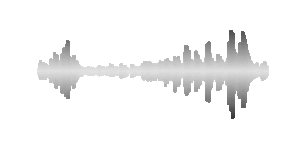
\includegraphics[scale=.5]{WaveformWithoutBg}
            \end{textblock*}
            \begin{figure}
                \centering
								\begin{footnotesize}
									\begin{picture}(96,26)
										\setcounter{iXOffset}{0}
										\setcounter{iYOffset}{5}
										\setcounter{iXBlockSize}{28}
										\setcounter{iYBlockSize}{16}
										\setcounter{iYBlockSizeDiv2}{8}
										\setcounter{iDistance}{8}

										\addtocounter{iYOffset}{\value{iYBlockSizeDiv2}}
										\addtocounter{iYOffset}{-2}

										%\addtocounter{iXOffset}{-1}
										\put(\value{iXOffset}, \value{iYOffset})
											{\text{{\shortstack[c]{audio\\ signal}}}}
										\addtocounter{iXOffset}{1}

										\addtocounter{iYOffset}{2}
										\addtocounter{iXOffset}{\value{iDistance}}

										\put(\value{iXOffset}, \value{iYOffset})
											{\vector(1,0){\value{iDistance}}}

										\addtocounter{iXOffset}{\value{iDistance}}
										\addtocounter{iYOffset}{-\value{iYBlockSizeDiv2}}
										
										\put(\value{iXOffset}, \value{iYOffset})
											{\framebox(\value{iXBlockSize}, \value{iYBlockSize}) {\shortstack[c]{feature extraction}}}

										\addtocounter{iXOffset}{\value{iXBlockSize}}
										\addtocounter{iYOffset}{\value{iYBlockSizeDiv2}}

										\put(\value{iXOffset}, \value{iYOffset})
											{\vector(1,0){\value{iDistance}}}

										\addtocounter{iXOffset}{\value{iDistance}}
										\addtocounter{iYOffset}{-\value{iYBlockSizeDiv2}}

										\put(\value{iXOffset}, \value{iYOffset})
											{\framebox(\value{iXBlockSize}, \value{iYBlockSize}) {\shortstack[c]{classification,\\ inference}}}

										\addtocounter{iXOffset}{\value{iXBlockSize}}
										\addtocounter{iYOffset}{\value{iYBlockSizeDiv2}}

										\put(\value{iXOffset}, \value{iYOffset})
											{\vector(1,0){\value{iDistance}}}

										\addtocounter{iXOffset}{\value{iDistance}}
										\addtocounter{iYOffset}{-2}

										\addtocounter{iXOffset}{1}
										\put(\value{iXOffset}, \value{iYOffset})
											{\text{{\shortstack[c]{class\\ labels}}}}
										
									\end{picture}
								\end{footnotesize}
            \end{figure}
            
            \vspace{-5mm}
            \begin{columns}
                \column{.5\textwidth}
                    \begin{itemize}
                        \item<2->[]	\textbf{feature} representation
                                \begin{itemize}
                                    \item 	compact and non-redundant
                                    \item	task-relevant
                                    \item   easy to analyze
                                    \item   e.g., MFCCs etc.
                                \end{itemize}
                    \end{itemize}
                \column{.5\textwidth}
                    \begin{itemize}
                        \item<3->[]	\textbf{classification}
                                \begin{itemize}
                                    \item	map or convert feature to comprehensible domain
                                    \item   e.g., Support Vector Machines etc.
                                \end{itemize}
                    \end{itemize}
            \end{columns}
            \phantom{\footfullcite{burred_hierarchical_2004}}
        \end{frame}
        
        \begin{frame}{introduction}{neural network based approaches}
            \vspace{-3mm}
            \begin{itemize}
                \item   no custom-designed features anymore
                \item   learn features from basic inputs (like spectrograms)
            \end{itemize}
            \begin{figure}%
                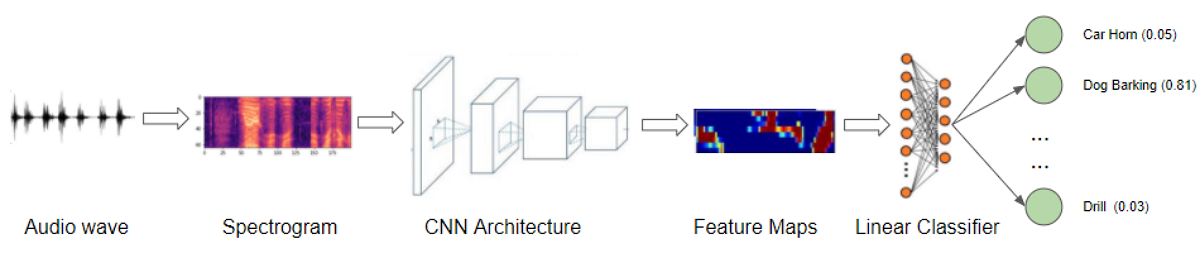
\includegraphics[width=\columnwidth]{audio_classification}%
            \end{figure}
            \addreference{Fig.: \href{https://towardsdatascience.com/audio-deep-learning-made-simple-sound-classification-step-by-step-cebc936bbe5}{towardsdatascience.com}}
            \pause
            \begin{itemize}
                \item   less required expert-knowledge, more complex systems
                \item   less expert-tweaking, more rigorous experimental requirement
                \item   much \textcolor{gtgold}{\textbf{higher data requirements}}
            \end{itemize}
            
        \end{frame}
